% Options for packages loaded elsewhere
\PassOptionsToPackage{unicode}{hyperref}
\PassOptionsToPackage{hyphens}{url}
%
\documentclass[
]{standalone}
\usepackage{lmodern}
\usepackage{amssymb,amsmath}
\usepackage{ifxetex,ifluatex}
\usepackage{tikz}
\usepackage{enumerate}
\usepackage{hyperref}
\usepackage[margin=0.75in]{geometry}
\usetikzlibrary{arrows,positioning,calc}


% \title{Raft Reconfig Bug (Single Node Change)}
% \author{William Schultz}

\begin{document}
% \maketitle

% \begin{enumerate}[(1)]
%     \item \textbf{One add, one remove}:
    
    
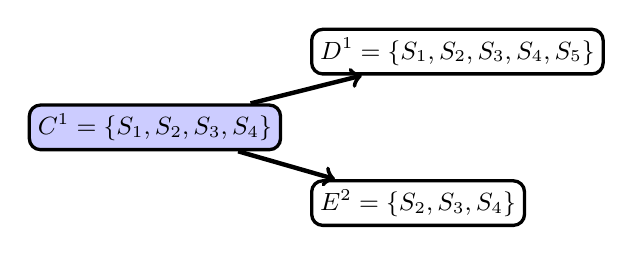
\begin{tikzpicture}
[scale=.5,auto=left,every node/.style={circle,fill=blue!20,minimum size=1pt}]
\small

%   \node[circle, draw=black, very thick,fill=red!20] (Ca) at (0,0) {$C_{0,0}$};
\node[rounded corners,rectangle, draw=black, very thick] (Ci)  {$C^1=\{S_1,S_2,S_3,S_4\}$};
\node[rounded corners,rectangle, draw=black, very thick,fill=white, above right=0.5cm of Ci] (Cs)  {$D^1=\{S_1,S_2,S_3,S_4,S_5\}$};
\node[rounded corners,rectangle, draw=black, very thick,fill=white!2,below right=0.5cm of Ci] (Cf) {$E^2=\{S_2,S_3,S_4\}$};
% \draw (Ca) edge[->,ultra thick] (Ci);
\draw (Ci) edge[->,ultra thick] (Cs);
\draw (Ci) edge[->,ultra thick] (Cf);
\end{tikzpicture}

% \item \textbf{Two adds}:
% \begin{center}
%     \begin{tikzpicture}
%     [scale=.5,auto=left,every node/.style={circle,fill=blue!20,minimum size=1pt}]
%     \small
    
%     %   \node[circle, draw=black, very thick,fill=red!20] (Ca) at (0,0) {$C_{0,0}$};
%     \node[rounded corners,rectangle, draw=black, very thick] (Ci)  {$C^1=\{S_1,S_2,S_3,S_4\}$};
%     \node[rounded corners,rectangle, draw=black, very thick,fill=white, above right=0.5cm of Ci] (Cs)  {$D^1=\{S_1,S_2,S_3,S_4,S_5\}$};
%     \node[rounded corners,rectangle, draw=black, very thick,fill=white!2,below right=0.5cm of Ci] (Cf) {$E^2=\{S_1,S_2,S_3,S_4,S_5,S_6\}$};
%     % \draw (Ca) edge[->,ultra thick] (Ci);
%     \draw (Ci) edge[->,ultra thick] (Cs);
%     \draw (Ci) edge[->,ultra thick] (Cf);
%     \end{tikzpicture}
% \end{center}

% \item \textbf{Two removes}:
% \begin{center}
%     \begin{tikzpicture}
%     [scale=.5,auto=left,every node/.style={circle,fill=blue!20,minimum size=1pt}]
%     \small
    
%     %   \node[circle, draw=black, very thick,fill=red!20] (Ca) at (0,0) {$C_{0,0}$};
%     \node[rounded corners,rectangle, draw=black, very thick] (Ci)  {$C^1=\{S_1,S_2,S_3,S_4\}$};
%     \node[rounded corners,rectangle, draw=black, very thick,fill=white, above right=0.5cm of Ci] (Cs)  {$D^1=\{S_1,S_2,S_3\}$};
%     \node[rounded corners,rectangle, draw=black, very thick,fill=white!2,below right=0.5cm of Ci] (Cf) {$E^2=\{S_1,S_2,S_4\}$};
%     % \draw (Ca) edge[->,ultra thick] (Ci);
%     \draw (Ci) edge[->,ultra thick] (Cs);
%     \draw (Ci) edge[->,ultra thick] (Cf);
%     \end{tikzpicture}
% \end{center}

% \end{enumerate}

\end{document}
